\documentclass{article}

% Encodings, page setup, paragraph formatting, font
\usepackage[top=0.9in, bottom=1in, left=1.5in, right=1.5in]{geometry}
\usepackage[utf8]{inputenc}
\usepackage[icelandic]{babel}
\usepackage[T1]{fontenc}
\usepackage[sc]{mathpazo}
\usepackage[parfill]{parskip}

% Tables and lists
\usepackage{booktabs,tabularx}
\usepackage{multirow}
\usepackage{enumerate}

% Math
\usepackage{amsmath, amsfonts, amssymb, amsthm}

% Graphics
\usepackage{graphicx}
\usepackage{tikz}

% Code environment
\usepackage{minted}

% Hyperlinks and related
\usepackage[bookmarks=true,colorlinks=true,pdfauthor={Magnús Pálsson},linkcolor=blue,urlcolor=blue]{hyperref}

% Minted configuration
\usemintedstyle{default}
\renewcommand{\theFancyVerbLine}{\sffamily \arabic{FancyVerbLine}}
\floatstyle{plaintop}
\newfloat{program}{thp}{lop}
\floatname{program}{Forrit}

% macros
\newcommand\norm[1]{\left\lVert#1\right\rVert}

% Meta information
\date{}
\author{Magnús Pálsson}
% Hyphenation
\hyphenpenalty=5000
% Page and section numbering
\setcounter{secnumdepth}{-1} 
\pagenumbering{gobble}
\usepackage{bm}


\title{Seismology \\ - \\ \large Homework 2}
\author{Magnús Pálsson}
\begin{document}
\maketitle

\section*{Problem 1}
Assume that the horizontal components of the 2-D stress tensor are
\begin{equation*}
\boldsymbol{\tau} = 
    \begin{bmatrix}
        \tau_{xx} & \tau_{xy} \\
        \tau_{yx} & \tau_{yy}
    \end{bmatrix}
    =
    \begin{bmatrix}
        -30 & -20 \\
        -20 & -40
    \end{bmatrix}
    \text{MPa}
\end{equation*}

\textbf{(a)} Compute the normal and shear stresses on a fault that strikes 10° east of north.

\textbf{(b)} Compute the principal stresses, and give the azimuths (in degrees east of north) of the maximum and minimum compressional stress axes.

\subsection*{(a) Solution}
We have 
\begin{equation*}
    \hat{\mathbf{n}} = 
    \begin{bmatrix}
        \cos(10^{\circ}) \\
        -\sin(10^{\circ})
    \end{bmatrix}
    \approx 
    \begin{bmatrix}
        0.9848 \\
        -0.1736
    \end{bmatrix}
\end{equation*}
And 
\begin{equation*}
    \mathbf{t}(\hat{\mathbf{n}}) = \boldsymbol{\tau}\hat{\mathbf{n}} \approx
    \begin{bmatrix}
        -30 & -20 \\
        -20 & -40
    \end{bmatrix}
    \begin{bmatrix}
        0.9848 \\
        -0.1736
    \end{bmatrix}
    \approx
    \begin{bmatrix}
        -26.0713 \\
        -12.7502
    \end{bmatrix}
\end{equation*}
This gives us 
\begin{equation*}
    t_N = \mathbf{t}(\hat{\mathbf{n}}) \cdot \hat{\mathbf{n}} \approx 
    \begin{bmatrix}
        -26.0713 \\
        -12.7502
    \end{bmatrix}
    \cdot
    \begin{bmatrix}
        0.9848 \\
        -0.1736
    \end{bmatrix}
    \approx -23.4611
\end{equation*}
And 
\begin{equation*}
    t_S = \sqrt{\norm{\mathbf{t}(\hat{\mathbf{n}})}^2 - t_N^2} \approx 17.0837
\end{equation*}


\subsection*{(b) Solution}

To find the principal stresses we need the eigenvalues of $\boldsymbol{\tau}$. Using Python we find them to be $\lambda_1 = -55.6155$ and $\lambda_2 = -14.3845$. The associated eigenvectors are 
\begin{equation*}
    \mathbf{u}^{(1)} \approx
    \begin{bmatrix}
        0.6154 \\
        0.7882
    \end{bmatrix}
    , \quad \text{and} \quad
    \mathbf{u}^{(2)} \approx
    \begin{bmatrix}
        0.7882 \\
        -0.6154
    \end{bmatrix}
\end{equation*}

The azimuth in degrees east of north of the maximum compressional stress axis is 
\begin{equation*}
    \sin^{-1}\left( \frac{\mathbf{u}^{(1)}_x}{\norm{\mathbf{u}^{(1)}}} \right) \approx
    \sin^{-1}\left(\frac{0.6154}{1}\right) \approx 
    \sin^{-1}\left( 0.6154\right) = 37.9819^{\circ}
\end{equation*}
As for the minimum compressional stress axis it will be perpendicular to the maximum compressional stress axis and inspection reveals that the azimuth in degrees east of north is $37.9819^{\circ} + 90^{\circ} = 127.9819$
\pagebreak
\section*{Problem 2}

Figure 3.6 in Shearer plots a harmonic plane wave at $t=0$, traveling in the x direction at 5 km/s.

\textbf{(a)} Write down an equation for this wave that describes displacement $\mathbf{u}$ as a funciton of $x$ and $t$

\textbf{(b)}

\textbf{(c)}

\textbf{(d)} What is the maximum strain for this wave?

\subsection*{Solution (a)}

We are looking to write the wave in the form $\mathbf{u}(x,t) = A\sin(\omega t - kx)$. We choose sin because the wave is 0 at $t = 0, x = 0$.

From the figure we can see that $A = 0.04$, $\lambda = 8000$m, and $v = 5000$m/s\\
Now we can calculate the period $T = \frac{\lambda}{v} = \frac{8000}{5000} = 1.6$s, the angular velocity $\omega = \frac{2\pi}{T} = \frac{5}{4}\pi = 1.25\pi \text{s}^{-1}$ and the wave number $k = \frac{2\pi}{\lambda} = 2.5\times 10^{-4}\pi$. So we have the equation
\begin{equation*}
    \mathbf{u}(x,t) = 0.04\sin(1.25\pi t - 2.5\times 10^{-4}\pi x)
\end{equation*}

\subsection*{Solution (b)}
$\sin(x) = cos(x - \frac{\pi}{2})$. So we can write 
\begin{equation*}
    \mathbf{u}(x,t) = 0.04\cos(1.25\pi t - 2.5\times 10^{-4}\pi x - \frac{\pi}{2})
\end{equation*}

Why we would do this is beyond me

\subsection*{Solution (c)}

We plug in

\begin{align*}
    \mathbf{u}(6000,30) &= 0.04\sin(1.25\pi 30 - 2.5\times 10^{-4}\pi 6000)\\
    &= 0.04\sin(\frac{150}{4} \pi - \frac{6}{4}\pi) \\
    &= 0.04\sin(\frac{144}{4}\pi) = 0.04\sin(36\pi) = 0
\end{align*}

\subsection*{Solution (d)}

Due to $\mathbf{u}(x,t)$ having only one spatial dimension we only need to calculate 
\begin{align*}
    \mathbf{e}_{xx} &= \frac{\partial \mathbf{u}(x,t)}{\partial x}\\
    &= 0.04 * (-2.5 \times 10^{-4}\pi) \cos(1.25\pi t - 2.5\times 10^{-4}\pi x)\\
    &=- \pi \times 10^{-5} \cos(1.25\pi t - 2.5\times 10^{-4}\pi x)
\end{align*}

Given that cosine takes values on $[-1,1]$. This funciton achieves the maximum of $kA = \pi \times 10^{-5}$
\pagebreak
\section*{Problem 3}
Consider two types of monochromatic plane waves propagating in the x direction in a uniform medium: 

\textbf{(a)} $P$ wave in which $u_x = A\sin(\omega t-kx)$,

\textbf{(b)} $S$ wave with displacements in the $y$ direction, i.e., $u_y = A\sin(\omega t-kx)$

For each case, derive expressions for the non-zero components of the stress tensor.

\subsection*{Solution (a)}

Of all the partial derivatives of $\mathbf{u}$, only the x derivative of the x component $\partial_x u_x = -kA\cos(\omega t-kx)$ is non-zero. We will avoid writing out the full expression to save space, writing the strain and stress in terms of $\partial_x u_x$. We get the strain tensor:

\begin{equation*}
    \mathbf{e} = 
    \begin{bmatrix}
        \partial_x u_x & \frac{1}{2}\partial_x u_x & \frac{1}{2}\partial_x u_x \\
        \frac{1}{2}\partial_x u_x & 0 & 0\\
        \frac{1}{2}\partial_x u_x & 0 & 0
    \end{bmatrix}
\end{equation*}

We see that $\text{tr}(\mathbf{e}) = \partial_x u_x$ so eqn. 2.30 from Shearer gives us the stress tensor:

\begin{equation*}
    \boldsymbol{\tau} = 
    \begin{bmatrix}
        (\lambda + 2\mu) \partial_x u_x & \mu \partial_x u_x & \mu \partial_x u_x\\
        \mu \partial_x u_x  & \lambda \partial_x u_x & 0 \\
        \mu \partial_x u_x & 0 & \lambda \partial_x u_x 
    \end{bmatrix}
    = \partial_x u_x 
    \begin{bmatrix}
        (\lambda + 2\mu) & \mu  & \mu \\
        \mu   & \lambda & 0 \\
        \mu  & 0 & \lambda 
    \end{bmatrix}
\end{equation*}

\subsection*{Solution (b)}

For the S wave, only the y component of $\mathbf{u}$ is non-zero and it only depends on x. Therefore, of the partial derivatives of the components of $\mathbf{u}$, only $\partial_xu_y = -kA\cos(\omega t-kx)$ is non-zero. This gives us the strain tensor:

\begin{equation*}
    \mathbf{e} = 
    \begin{bmatrix}
        0 & \frac{1}{2}\partial_x u_y & 0 \\
        \frac{1}{2}\partial_x u_y & 0 & 0\\
        0 & 0 & 0
    \end{bmatrix}
\end{equation*}

We see that $\text{tr}(\mathbf{e}) = 0$ so eqn. 2.30 from Shearer gives us the stress tensor:

\begin{equation*}
    \boldsymbol{\tau} = 
    \begin{bmatrix}
        0 & \mu\frac{1}{2}\partial_x u_y & 0 \\
        \mu\frac{1}{2}\partial_x u_y & 0 & 0\\
        0 & 0 & 0
    \end{bmatrix}
\end{equation*}
\pagebreak
\section*{Problem 7}
We use the code from the book as a guide and flesh out the following script

\inputminted{python}{P7script.py}

\pagebreak

The output images are as follows
\begin{figure*}[h]
    \centering
    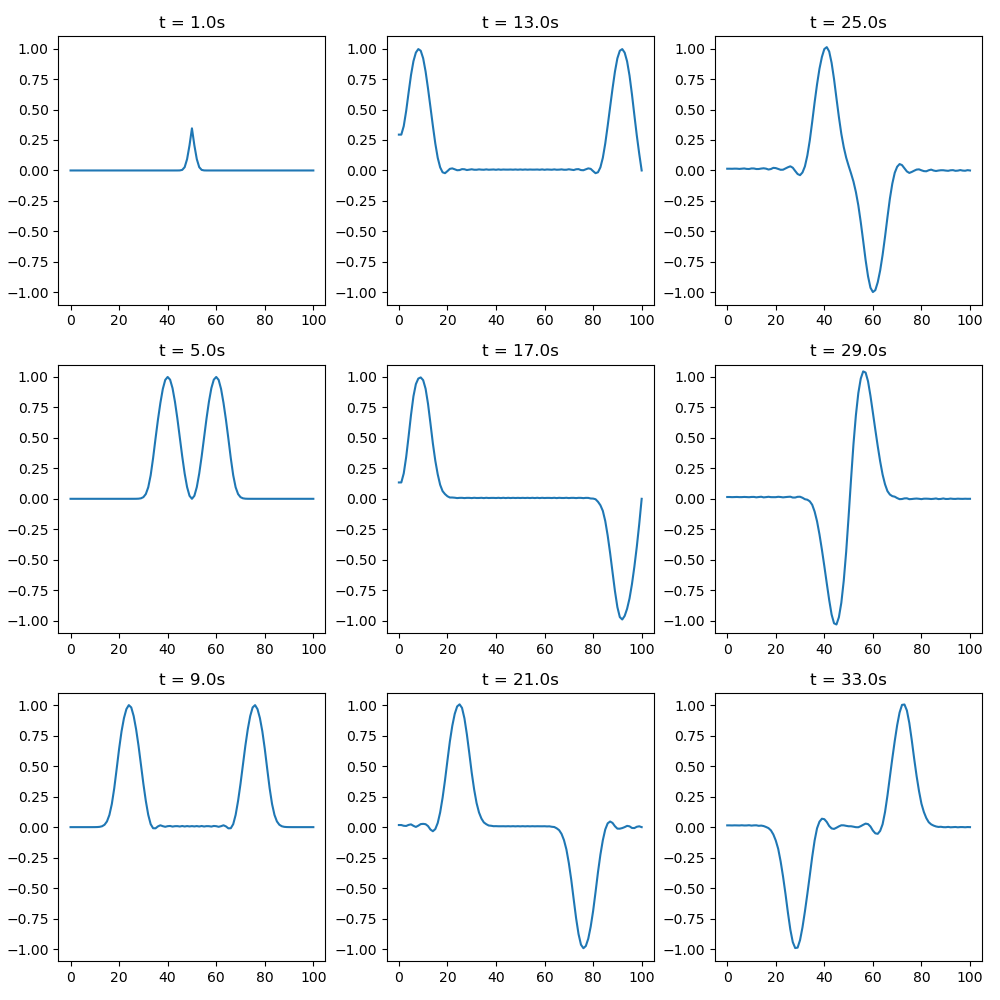
\includegraphics[scale=0.55]{figures/P7output}
\end{figure*}

We see that The pulse hitting the stress free boundary is reflected as is but the pulse hitting the fixed boundary has its displacement mirrored as it is reflected back. When the pulses meet they pass through each other.
\end{document}